% Extracted from higherOrderDerivativesAndGraphs.tex, problem #9
\begin{problem}
	Suppose the function $f$ has derivative given by $\displaystyle f'(x) = \dfrac{2x}{4+x^2}$.

	\begin{enumerate}
	
	%part a
	\item  Find a formula for $f''(x)$.
\WkstHop
			\begin{freeResponse}
				The second derivative is given by $\displaystyle f''(x) = \dfrac{2(4-x^2)}{(4+x^2)^2}$.
			\end{freeResponse}
			
			
			
	%part b
	\item  Construct a sign-chart for $f'$ and $f''$.
\WkstHop[2]
		\begin{freeResponse}
			For $f'$ we obtain:

			\begin{tikzpicture} 
				\tkzTabInit[lgt=2,espcl=1] 
					{$x$         /1, 
					$2x$   /1, 
					$4+x^2$ /1, 
					$f'(x)$      /1}% 
					{   , $0$ ,  }% 
				\tkzTabLine{ , - , t , + ,}
				\tkzTabLine{ , + , t , + ,}
				\tkzTabLine{ , - , t , + ,}
			\end{tikzpicture} 
			
			For $f''$, using the factorization $4-x^2 = (2+x)(2-x)$ , we obtain:			

			\begin{tikzpicture} 
				\tkzTabInit[lgt=2,espcl=1] 
					{$x$         /1, 
					$2$   /1, 
					$2+x$  /1,
					$2-x$  /1,
					$(4+x^2)^2$   /1, 
					$f''(x)$    /1}% 
					{  , $-2$ ,$2$,  }% 
				\tkzTabLine{  , + , t , + , t , + ,}
				\tkzTabLine{  , - , t , + , t , + ,}
				\tkzTabLine{  , + , t , + , t , - ,}
				\tkzTabLine{  , + , t , + , t , + ,}
				\tkzTabLine{  , - , t , + , t , - ,}
			\end{tikzpicture} 
		\end{freeResponse}
			
			
			
	%part c
	\item  On what interval(s) is $f$ increasing? On what interval(s) is $f$ concave down?
\WkstHop

			\begin{freeResponse}
				From the sign-chart for $f'$, we see that $f'$ is positive on $(0,\infty)$ 
				and negative on $(-\infty, 0)$.  We know that $f$ is increasing on an interval if $f'$ is positive on that interval. 
				That means: $f$ is increasing on the interval $(0,\infty)$.

				From the sign-chart for $f''$, we see that $f'$ is positive on $(-2,2)$ 
				and negative on $(-\infty, -2)$ and $(2, \infty)$.  We know that $f$ is concave down on an interval if $f''$ is negative on that interval. 
				That means: $f$ is concave down on the intervals $(-\infty, -2)$ and $(2,\infty)$.
			
			\end{freeResponse}
			
			
			
	\end{enumerate}
			
			
			
		
\end{problem}
